\section{Implementierung}
\label{sec: implementation}
In dieser Sektion wird sich ausgiebig mit der Implementierung der zuvor festgelegten Anforderungen auseinandergesetzt.

\subsection{Server}
\label{sec: server}
Da zu diesem Zeitpunkt bereits Librarys zur Authentifizierung existieren, wurde sich beginnend mit der Library Devise auseinandergesetzt.

\subsubsection{Devise}
\label{sec: devise}
Devise ist eine Ruby on Rails Library mit der sich eine flexible Authentifizierung ermöglichen lässt. Es bietet ein vorgefertigtes Datenbankschema für registrierte Benutzer, einen leichten Umgang mit OmniAuth und Funktionen wie beispielsweise das Senden einer E-Mail bei Registrierung. Im Datenbankschema enthalten ist ein Log-System mit dem zum Beispiel der Zeitpunkt der letzten Anmeldung eines Benutzers festgehalten werden kann. 

Die Funktionalitäten die Omniauth bietet sind jedoch für die Zielverwirklichung ausreichend, we{\ss}halb sich gegen Devise entschieden wurde. Aus diesem Grund mussten Funktionen wie zum Beispiel das Senden einer Bestätigungsmail selbst implementiert werden. 

\subsubsection{Omniauth}
\label{sec:omniauth}
Omniauth ist eine quelloffene Library für Ruby on Rails und ermöglicht dem Benutzer, eine Anmeldung mittels unterschiedlicher Anbieter über \gls{oAuth2}. Bei der Anmeldung mittels oAuth2 werden bereits viele Funktionen von Omniauth selber übernommen. Sobald der Nutzer sich bei dem jeweiligen Anbieter angemeldet hat, wird die Antwort des jeweiligen Anbieters automatisch über die von Omniauth festgelegte Route verarbeitet. Jedoch muss vorher das spezifische Gem des Anbieters für Omniauth installiert werden. Hierbei stellt jedes Gem eine eigene Strategie für Omniauth bereit. Eine Strategie stellt die Möglichkeit bereit, sich mit einem speziellen Provider zu authentifizieren.

Omniauth selber verfügt nur über die Developer Strategie, diese ermöglicht eine Anmeldung ohne spezifische Überprüfung der angegebenen Daten. Das hat zur Folge, dass diese Art von Anmeldung auf keinen Fall im Produktiv System vorhanden sein darf.

Den Vorteil, den Omniauth bietet, ist die Kapselung zwischen den spezifischen Providern und der Hauptfunktionalität von Omniauth. Dementsprechend kann der Server nur explizit mit den installierten Providern kommunizieren. Zudem bietet Omniauth eine lange Liste an zu installierenden Providern.

Beispiele an zu installierenden Providern: 
\begin{enumerate} 
	\item GitHub\footnote{https://github.com/omniauth/omniauth-github}
	\item GitLab\footnote{https://github.com/linchus/omniauth-gitlab}
	\item Goodreads\footnote{https://github.com/sandboxws/omniauth-goodreads}
	\item Google\footnote{https://github.com/Yesware/omniauth-google}
\end{enumerate}

\subsubsection{Pundit}
\label{sec: pundit}
Pundit ist eine Ruby on Rails Library die ein Designpattern zur Autorisierung bietet. Bei diesem Pattern werden zu einem jeweiligen Controller eine Policy angelegt. Eine Policy ist hierbei nur eine Klasse. Dabei setzt sich der Name der Policy, aus dem Namen des Models und dem Schlüsselwort Policy als Suffix zusammen. Dem Konstruktor der Policy wird beispielsweise ein Nutzer und das jeweilige Objekt übergeben, welches auf den Zugriff geprüft werden soll. Innerhalb der Policy werden die jeweiligen Controllerfunktionsköpfe, in denen eine Autorisierung stattfinden soll, mit einem \enquote{?} als Suffix ergänzt und definiert. Diese Funktionen müssen zwingend einen Boolean als Rückgabewert erhalten, um eine gültige Auswirkung als Policy zu haben. Sobald die aufgerufene Funktion der Policy fehlschlägt, wird eine Exception geworfen. Diese Exception kann an jeweiliger Position beispielsweise im Controller abgefangen und verarbeitet werden.

Da es sich bei Policies um Klassen handelt, können diese auch instanziiert und die jeweiligen Funktionen dynamisch abgerufen werden. Dies hat zur Folge, dass explizit nach einer bestimmten Policy-Funktion gefragt werden kann, selbst wenn der Funktionsname nicht dem der aufgerufenen Policy-Funktion entspricht.

\subsubsection{Rolify}
\label{sec: rolify}
Rolify ist eine Ruby on Rails Library zur Verwaltung von Rollen. Hierbei liefert Rolify bereits zwei Datenbanktabellen im Design der polymorphen Assoziation (Abbildung \ref{fig:server-polymorph-association}). Bei einer Eins-zu-viele-Assoziation hat beispielsweise ein Nutzer verschiedene Rollen, die verschiedene Fremdschlüssel aus verschiedenen Tabellen beinhalten. Dabei ergibt sich das Problem, dass nicht mehr sicher gestellt werden kann aus welcher Tabelle der Fremdschlüssel stammt. Um dieses Problem zu lösen gibt es drei bewährte Methoden. In dieser Thesis gehen wir jedoch nur auf die von Rolify mitgelieferte Methode ein.

Bei dieser Methode handelt es sich um eine Kindtabelle \enquote{roles} und einer Elterntabelle \enquote{users\_roles}. Dabei stehen in der Roles-Tabelle die jeweiligen Informationen der Rolle und auf welche Ressource diese Rolle sich bezieht. Rolify unterscheidet hierbei zwischen globalen und ressourcenspezifische Rollen. Eine globale Rolle beinhaltet keine Informationen einer Ressource und kann da zum Beispiel als allgemeine \enquote{user} Rolle dienen.

\begin{figure}[h]
	\centering
	\includegraphics[width=.6\textwidth]{graphics/rolify.pdf}
	\caption{Rolifys Datenbanktabellen mit Beziehung zur users Tabelle}
	\label{fig:server-polymorph-association}
\end{figure}

Die \enquote{users\_roles} beinhaltet wiederum die jeweilige \enquote{user\_id} und die zu dem Nutzer dazugehörigen Primärschlüssel einer Rolle. Dabei können verschiedene Nutzer dieselbe Rolle, als auch verschiedene Rollen haben.

Dem zuzüglich liefert Rolify bereits vordefinierte Funktionen, mit denen es möglich ist, jeweilige Rollen eines Nutzers abzufragen, hinzuzufügen oder zu entfernen.



\subsubsection{Anmeldung eines Benutzers}
\label{sec: sign-in-imp}
Die Anmeldung mittels oAuth2 oder Passwort wurde mit Omniauth ermöglicht. Hierbei wurde zuerst Omniauth selber dem derzeitigen Projekt hinzugefügt und darauffolgend die Gems zur Authentifizierung mittels Google, GitHub und Passwort. Um die einzelnen Provider nutzen zu können, müssen diese in einem \enquote{initializer} (Listing \ref{lst:added_providers}) deklariert werden. Ein \enquote{initializer} wird nach dem Rails Framework und den dazugehörigen Gems geladen. Bei der Deklarierung der Provider ist zu beachten, dass Provider wie Google oder GitHub eine jeweilige ID und einen Secret-Key als Parameter benötigen. Diese werden jeweils auf den offiziellen Seiten der Provider erstellt. Dabei musste darauf geachtet werden, dass diese ID und dieser Secret-key über eine Umgebungsvariable mit in das Projekt eingebunden wird. Umgebungsvariablen werden in dem Fall in der Kommandozeile vor das Kommando zum Starten des Projektes gesetzt. Nachdem das Kommando zum starten des Servers ausgeführt wurde, kann auf die Werte der zuvor festgelegten Umgebungsvariablen zugegriffen werden. Die Verwendung von Umgebungsvariablen ist besonders bei Blattwerkzeug vonnöten, da es sich um ein quelloffenes Projekt handelt und jeder den bereits produzierten Code einsehen kann. Da es sich bei Secret-Keys um Passwörter handelt, sind diese nicht im Repository angegeben.  

\begin{minipage}{\textwidth}
	\lstinputlisting[language=Ruby, style=CodeView, basicstyle=\scriptsize, caption=Zu Omniauth hinzugefügte Provider, captionpos=b, label={lst:added_providers}]{snippets/omniauth-initializer.rb}
\end{minipage}

Bei der Erstellung des User und des Identity Models wurde zuerst diskutiert, welche Attribute die jeweiligen Models haben sollten. Hierbei steht das Identity Model für alle hinzugefügten Authentifikations-Möglichkeiten eines Benutzers. Dabei wurde darauf geachtet, welche Attribute später dem Client zur Verfügung gestellt und welche für spätere Controller Funktionen benötigt werden.

\subsubsection*{Attribute der identities Tabelle}
Die nachfolgenden Beschreibungen der Attribute beziehen sich auf die identities Tabelle, welche in Abbildung \ref{fig:server-users-identities} dargestellt wird.
\begin{description}
	\item[uid]\hfill\\
	Die uid ist ein String, der zur eindeutigen Identifikation des Kontos eines Providers dient. Dabei kann die uid zum Beispiel eine Zahl oder eine E-Mail sein. Mit der uid wird festgestellt, ob ein bestimmtes Konto bereits mit einem Benutzer verknüpft ist.
	\item[provider]\hfill\\
	Das provider Attribut wird mit dem jeweiligen Provider-Namen beschrieben. Dabei sind die Namen, wie in Listing \ref{lst:added_providers} definiert. Da die Namen jedoch von den installierten Gems definiert werden, ist eine Änderung dieser Namen nicht ohne weiteres Möglich.
	\item[provider\_data]\hfill\\
	Das provider\_data Attribut wird mit jeglichen Daten beschrieben, die ein Provider über den authentifizierten Benutzer zurückliefert. (Listing \ref{lst:server-github-oauth-data} \& \ref{lst:server-google-oauth-data})
	
	\begin{minipage}{.42\textwidth}
		\lstinputlisting[language=JSON, style=CodeView, basicstyle=\scriptsize, caption=GitHubs oAuth Daten, captionpos=b, label={lst:server-github-oauth-data}]{snippets/github-provider-data.json}
	\end{minipage}\hfill
	\begin{minipage}{.42\textwidth}
		\lstinputlisting[language=JSON, style=CodeView, basicstyle=\scriptsize, caption=Googles oAuth Daten, captionpos=b, label={lst:server-google-oauth-data}]{snippets/google-provider-data.json}
	\end{minipage}
	
	\item[own\_data]\hfill\\
	Das own\_data Attribut wird mit den Daten beschrieben, die Blattwerkzeug für den Benutzer vorgesehen hat. Dies kann beispielsweise der Token zur Aktivierung einer E-Mail sein.
	\item[type]\hfill\\
	Das type Attribut wird, sobald es der Tabelle hinzugefügt wurde, von Rails automatisch interpretiert. Hierbei handelt es sich um \gls{STI}. \gls{STI} stellt eine Möglichkeit der Objekt-Orientierung in einer Relationellen Datenbank zu emulieren. Dabei ist die Tabelle identities und dessen Model (Identity) die Basisklasse und die in type festgelegten Klassen, die Abgeleiteten. Das type Attribut ermöglicht einen sofortigen Zugriff auf die Klasse des Providers einer ausgewählten Identity.
\end{description}

\begin{figure}[h]
	\centering
	\includegraphics[width=0.65\textwidth]{graphics/users-identities.pdf}
	\caption{Darstellung der users und identities Tabelle inklusive Beziehung.}
	\label{fig:server-users-identities}
\end{figure}

\subsubsection*{Attribute der users Tabelle}
Die nachfolgenden Beschreibungen der Attribute beziehen sich auf die users Tabelle, welche in Abbildung \ref{fig:server-users-identities} dargestellt wird.
\begin{description}
	\item[display\_name]\hfill\\
	Das display\_name Attribut steht für den Anzeigenamen des Benutzers. Dieser ist jedoch nicht einzigartig und lässt sich beliebig oft verändern. Das hat zur Folge, dass mehrere Benutzer denselben Anzeigenamen haben können.
	\item[email]\hfill\\
	Das email Attribut steht für die primäre E-Mail eines Benutzers. Die primäre E-Mail wird verwendet, sobald eine E-Mail von Blattwerkzeug an den Benutzer gesendet wird. Dies ist wichtig, da jedes verknüpfte Konto eine unterschiedliche E-Mail besitzen darf. Die primäre E-Mail wird bei Erstellung eines Benutzers gesetzt, au{\ss}er ein Benutzer authentifiziert sich über einen Provider, dessen Rückgabe keine E-Mail enthält.
\end{description}


\subsubsection{Anmeldung mittels \gls{oAuth2}}
\label{sec:sever-sign-in-oauth2}
Bei einer Anmeldung mittels \gls{oAuth2} wurde bei dem Provider, über den sich authentifiziert wird, eine Redirect Url hinterlegt. Auf diese wird der jeweilige Benutzer nach Authentifikation zurückgeleitet. Die Route zu der Redirect Url zeigt auf die Funktion mit dem Namen \enquote{callback} im \enquote{AuthController}. Die callback Funktion prüft auf das Vorhandensein der vom Provider zurückgelieferten Daten. Sollte bisher keine Identität mit den Daten des Providers erstellt worden sein wird eine neue Identität angelegt. Führt ein angemeldeter Benutzer diese Funktion aus, wird ihm eine neue Identität zu seinem Konto hinzugefügt. Handelt es sich nicht um einen angemeldeten Benutzer, wird zusätzlich ein neuer Benutzer erstellt. Da jeder Provider unterschiedliche Daten zurückliefert, wird bei dem Anlegen einer neuen Identität zwischen den einzelnen Providern unterschieden. Jeder Provider besitzt eine Abgeleiteteklasse der Basisklasse Identity und greift innerhalb seiner Klasse auf die für ihn relevanten Daten zu. Sollte eine Identität mit den zuürckgelieferten Daten bereits existieren, wird ohne Erstellung einer Identität fortgefahren. Mit der erstellten oder existierenden Identität werden die Benutzerinformationen in die Payload eines \gls{JWT} geschrieben. Bei den Benutzerinformationen handelt es sich um die id, den display\_name und die Rollen eines Benutzers. Die Funktionen zu Erstellung eines \gls{JWT} wurden hierbei in einen Helper ausgelagert und die Gültigkeitsdauer des erstellten \gls{JWT} beläuft sich auf eine Stunde.

\begin{figure}[h]
	\centering
	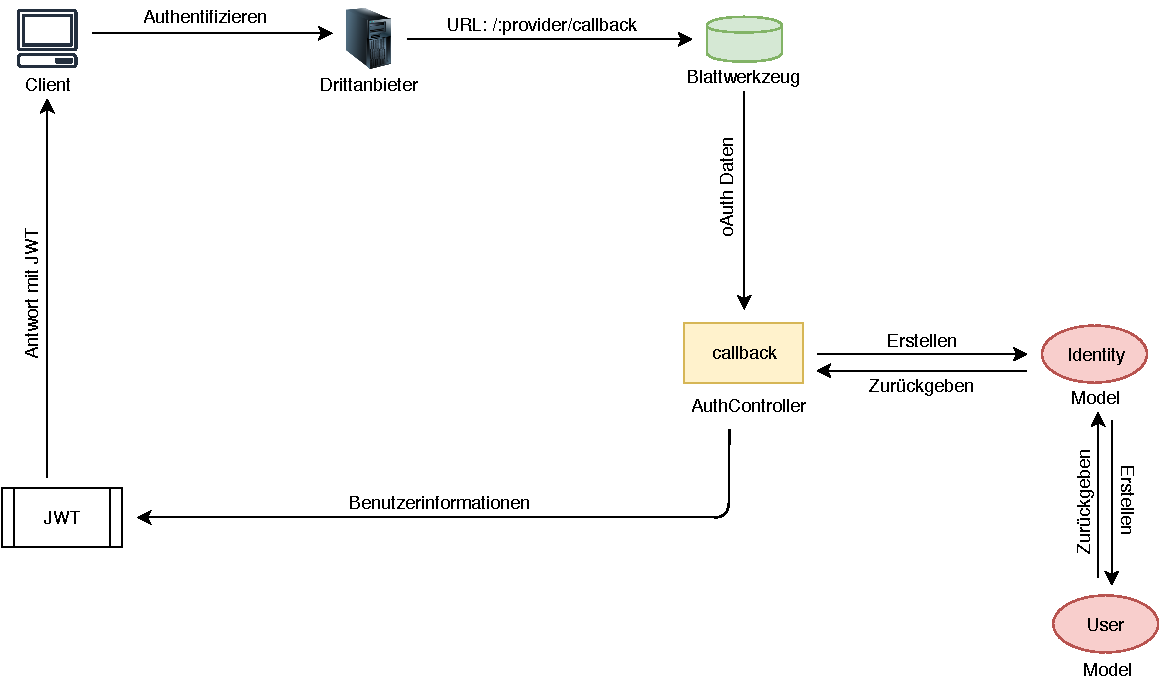
\includegraphics[width=0.8\textwidth]{graphics/sign-in-oauth2.pdf}
	\caption{Ablauf einer Anmeldung mittels \gls{oAuth2}}
	\label{fig:server-sign-in-oauth}
\end{figure}

\subsubsection{Anmeldung mittels Passwort}
\label{sec:sever-sign-in-password}
Die Anmeldung mittels Passwort wurde mittels Omniauth Identity\footnote{\url{https://github.com/omniauth/omniauth-identity}} ermöglicht. Omniauth Identity ist ebenfalls eine Strategie mit der die Möglichkeit gegeben ist, sich über ein Passwort bei Blattwerkzeug anzumelden. Ebenso wie die Developer Strategie bietet auch diese Strategie die Möglichkeit, ein vorgefertigtes Formular für Anmeldung und Registrierung zu erstellen. Jedoch ist es bei dieser Strategie optional, und eine ausschlie{\ss}liche Kommunikation über ein API ist möglich.

Bei dem Nutzen dieser Strategie fiel auf, dass die Daten übermittelt wurden sie jedoch nicht richtig verarbeitet werden konnten (Listing \ref{lst:register_omniauth_identity}). Das hatte zur Folge, dass mit der Erstellung eines Models, welches mit als Parameter im iniziliazer angegeben werden kann, nicht ordnungsgemä{\ss} fortgefahren werden konnte. Um fortzufahren, wäre es möglich eine eigene Strategie für Omniauth zu entwickeln oder auf die von Omniauth Identity mitgelieferten Optionen zurück zugreiffen.

Omniauth Identity bietet die Möglichkeit bei der Registrierung auf eine Funktion zu verweisen. Diese Funktion muss ebenfalls im \enquote{initializer} angegeben werden. (Listing \ref{lst:added_providers}). Tritt bei der Erstellung des Models ein Fehler auf (Listing \ref{lst:register_omniauth_identity}), wird die Funktion, im zuvor festgelegten iniziliazer, aufgerufen. Letztendlich hat man sich in der Thesis für diese Methode entschieden. Hierbei werden jegliche Funktionen innerhalb des AuthControllers und au{\ss}erhalb der Strategie genutzt.


\begin{minipage}{\textwidth}
	\lstinputlisting[language=Ruby, style=CodeView, caption=Aufgerufene Funktion bei POST Request (Omniauth Identity), captionpos=b, label={lst:register_omniauth_identity}]{snippets/omniauth-identity-registration.rb}
\end{minipage}


\begin{description}
	\item[Registrierung]\hfill\\
	Bevor eine Anmeldung mittels Passwort stattfinden kann, wurde eine Registrierungs-Möglichkeit hinzugefügt. Die \enquote{register} Funktion arbeitet ähnlich, wie die callback (Sektion \ref{sec:sever-sign-in-oauth2}) Funktion. Der Unterschied besteht darin, dass die register Funktion einen simulierten Hash in der Struktur Omniauths erhält und mit diesem versucht, eine neue Identität zu erstellen. Bei dem Erstellen einer neuen Password-Identität wird ein Verifizierungs-Token generiert. Dieser Verifizierungs-Token ist eine \gls{UUID} und wird zur Verzifizierung der Identität genutzt. Nachdem eine Identität erstellt wurde, sendet der Server mithilfe der Basisklasse ActionMailer eine Bestätigungsmail. Diese Bestätigungsmail verhindert das Registrieren von willkürlichen E-Mail Adressen. Zudem wird  mit der Bestätigungsmail eine E-Mail Adresse auf ihre Existens geprüft. Die Bestätigungsmail besteht aus einem Hyperlink zu einer \gls{URL} Blattwerkzeugs in der der Verifizierungs-Token enthalten ist. Sobald dieser \gls{URL} besucht wird, wird die Indentität als bestätigt gekennzeichnet. Dies erfolgt durch das Setzen des confirmed Feldes im JSON Blob Attribut own\_data.
	
	\item[Verifizierungsmail nicht erhalten]\hfill\\
	Da es vorkommen kann, dass eine Verifizierungsmail nicht an der angegebene E-Mail ankommt, wurde hierfür eine Funktion im IdentitiesController geschrieben. Diese Funktion prüft die übermittelte E-Mail auf ihre Existens in der Blattwerkzeug-Datenbank und ob diese bereits verifiziert wurde. Sollte diese E-Mail nicht verifiziert sein, wird eine neue Verifizierungsmail versendet. Gleichzeitig wird jedoch auch eine Wartezeit von zwei Minuten im own\_data Attribut festgelegt. Die Wartezeit zum Versenden einer neuen Verifizierungsmail soll verhindern, dass eine E-Mail Adresse mit Verifizierungsmails überhäuft werden kann.
	
	\item[Anmeldung mit verifizierter E-Mail]\hfill\\
	Ist eine Identität mit einem Passwort bereits vorhanden, kann sich mit E-Mail und Passwort angemeldet werden. Bei der Anmeldung wird das Passwort zur angegebenen E-Mail überprüft. Zusätzlich wird geprüft, ob die E-Mail verifiziert wurde. Sollten diese Sicherheitsabfragen erfolgreich durchlaufen sein, wird wie bei der Anmeldung mittels \gls{oAuth2} ein \gls{JWT} ausgestellt, in dem die Benutzerinformationen gespeichert werden.
	
	\item[Passwort vergessen]\hfill\\
		Da im Laufe der Zeit die Möglichkeit besteht, dass Benutzer ihr Passwort vergessen haben, wurde hierfür eine Funktion im IdentitiesController erstellt. Damit ein Passwort zurück gesetzt werden kann, muss die übermittelte E-Mail Adresse als Passwort Identität vorhanden sein. Sollte die Identität vorliegen, wird ein password\_reset\_token erstellt. Dieser password\_reset\_token ist eine \gls{UUID} und wird im own\_data JSON Blob Attribut gespeichert. Ebenfalls zum own\_data Attribut wird ein Feld password\_reset\_token\_exp hinzugefügt. Dessen Wert beläuft sich auf die aktuelle Uhrzeit plus drei{\ss}ig Minuten. Nachdem die festgelegte Uhrzeit des password\_reset\_token\_exp Feldes überschritten wurde, kann der Zurücksetzungs-Token nicht mehr verwendet werden. Damit das Passwort trotzdessen zurückgesetzt werden kann, muss ein neuer Zurücksetzungs-Token angefordert werden. Die Ablaufzeit eines Zurücksetzungs-Tokens hat den Vorteil, dass, sollte beispielsweise ein Angreiffer Zugriff auf den Browserverlauf haben, dieser nicht die Möglichkeit erhält, das Passwort dieses Benutzers zu verändern. Die E-Mail, die beim Kennwort zurücksetzen versendet wird, wird an die primäre E-Mail verschickt und enthält einen Hyperlink zum Wiederherstellen des Passwortes. Der Hyperlink beinhaltet den password\_reset\_token. Nachdem ein neues Passwort ausgewählt wurde, wird von jeder Passwort-Identität des Benutzers das Passwort geändert.
\end{description}

Blattwerkzeug nutzt Subdomains zur Unterteilung verschiedener Sprachen. Dabei ergab sich das Problem, dass das Umleiten auf eine Basisurl, die \gls{CSRF} Protection von Rails ausgelöst hat. Somit ist es derzeit möglich, sich über die Subdomains anzumelden, jedoch wird zwischenzeitlich ein Fehler zurückgegeben.

\subsubsection{Autorisierung}
\label{sec:server-authorisation}
Sobald ein Benutzer angemeldet ist, wird bei jedem Request ein \gls{JWT} mit an den Server gesendet. Dieser wird serverseitig auf seine Gültigkeit geprüft. Hierbei prüft der Server, ob dieser \gls{JWT} seine Ablaufzeit nicht überschritten hat und ob der \gls{JWT} die Signatur des Servers beinhaltet. Diese Überprüfung authentifiziert einen Besucher als angemeldeten Benutzer und wird von der Library jwt\footnote{\url{https://github.com/jwt/ruby-jwt}} übernommen.

Das Muster der globalen Rollen welches bereits von Rolify (Sektion \ref{sec: rolify}) implementiert wurde, konnte genutzt werden um die Benutzer in ihrem Status zu unterteilen. 

\begin{description}
	\item[guest]\hfill\\
	Die guest Rolle wird einem einzigen Benutzer zugewiesen. Dieser Benutzer beschreibt einen unangemeldeten Besucher. Jedem der Blattwerkzeug besucht und sich nicht anmeldet, wird dieser Gast-Benutzer zugewiesen. Der Gast-Benutzer besitzt keine Möglichkeit, Änderungen, die über Bedienelemente ermöglicht werden, zu speichern oder zu löschen.
	\item[user]\hfill\\
	Die user Rolle stellt einen angemeldeten Benutzer dar. Sollte bei einer Identitäts Erstellung festgestellt werden, dass der aktuelle Benutzer keine Globale-Rolle admin oder user besitzt, wird automatisch die user Rolle hinzugefügt. Mit der user Rolle wird das Erstellen, Speichern und Löschen von Projekten ermöglicht. Dies bezieht sich jedoch nur auf eigene Projekte.
	\item[admin]\hfill\\
	Die admin Rolle stellt einen administrierenden Benutzer dar. Jegliche Operationen, die mit der user Rolle ausgeführt werden, können ebenfalls mit der admin Rolle ausgeführt werden. Darüberhinaus kann ein Benutzer mit der admin Rolle, jegliche Projekte bearbeiten und beschränkt sich nicht nur auf seine eigenen. Der Admin-Benutzer besitzt zusätzliche Funktionen mit denen er beispielsweise eine Neuigkeit, die clientseitig auf der Startseite angezeigt wird, erstellen kann.
\end{description}

Um den Zugriff auf das Verwalten eines Projektes oder einer News zu beschränken, wurde jeweils eine Policy (Listing \ref{lst:project_policy}) angelegt. Bei der Erstellung einer Policy fiel auf, dass es sinnvoller ist, den Ersteller einer News oder eines Projektes in der jeweiligen Tabelle mit zu hinterlegen. Dafür wurde ein neues Attribut owner der projects und news Tabelle hinzugefügt. Dieses owner Attribut ist ein Fremdschlüssel und bezieht sicht auf die users Tabelle. Die Beziehung, die folgedessen enstand ist, ist eine 1:n. Das bedeutet, ein Benutzer kann zum Beispiel verschiedene Projekte besitzen, jedoch ein Projekt nur einen Benutzer haben. Den Vorteil, den das Hinzufügen des owner Attributes hat, ist der direkte Zugriff auf die erstellten Projekte eines Benutzers. Ebenso kann zwischen einem Ersteller eines Projektes und einem Benutzer der eine Rolle zum Bearbeiten eines Projektes erhalten hat, unterschieden werden.

\begin{minipage}{\textwidth}
	\lstinputlisting[language=Ruby, style=CodeView, caption=Policy zur Autorisierung eines Zugriffs auf ein Projekt, captionpos=b, label={lst:project_policy}]{snippets/project_policy.rb}
\end{minipage}

Da Blattwerkzeug bereits eine Passwortabfrage eingebaut hatte (Listing \ref{lst:controller_function_before}), dessen Anmeldedaten sich aber auf user und user beschränkten, mussten diese durch die von Pundit mitgelieferte authorize (Listing \ref{lst:controller_function_after}) Methode ersetzt werden.

\begin{minipage}{\linewidth}
	\lstinputlisting[language=Ruby, caption=Controller-Funktion ohne Integrierung Pundits, style=CodeView, captionpos=b, label={lst:controller_function_before}]{snippets/controller_authorisation_before.rb}
\end{minipage}

\begin{minipage}{\linewidth}
	\lstinputlisting[language=Ruby, caption=Controller-Funktion mit Integrierung Pundits, style=CodeView, captionpos=b, label={lst:controller_function_after}]{snippets/controller_authorisation_after.rb}
\end{minipage}

\subsubsection{may\_perform}
\label{sec:server-may-perform}
Sobald man sich mit den Rollen beschäftigt, stellte sich die Frage, wie die Bedienelemente in Abhängigkeit von den Rollen Clientseitig angezeigt werden sollten. Hierbei ergab sich, ein eigenes Pundit (Sektion \ref{sec: pundit}) ähnliches Mustur zu implementieren oder den Server bei jedem Bedienelement zu fragen, ob der aktuelle Benutzer Zugriff auf das Bedienelement hat. In der Thesis wurde sich für den zweiten Weg entschieden, da bei einer zusätzlichen clientseitigen Überprüfung, Client und Server gepflegt werden müssten. Sollte es vorkommen, dass die Pflege des serverseitigen Teils vergessen wurde, stellt dieses ein Sicherheitsrisiko dar. Clientseitige Anwendungen werden auf dem Endgerät eines Benutzers ausgeführt. Infolgedessen, besteht die Möglichkeit, die Anwendung zu manipulieren.

Die serverseitige Überprüfung der Bedienelemente wurde mittels der may\_perform Funktion realisiert. Diese erhält vom Client eine Liste an Daten, in der jedes Element ein Bedienelement darstellt. In der may\_perform Funktion wird jedes Element der Liste durchlaufen und auf das Zugriffsrecht des aktuellen Benutzers geprüft. Dies geschieht in dem aus den übermittelten Daten eine Instanz einer Policy erstellt wird, die zu der jeweiligen Ressource, beispielsweise der Projekte (Listing \ref{lst:project_policy}), gehört. Hierbei wird die Funktion, die auf ihren Zugriff geprüft werden soll, ebenfalls vom Client mit an den Server gesendet. Diese wird letztendlich auf der erstellten Instanz ausgeführt. Das Ergebnis der aufgerufenen Policy Funktion wird in einem Array gespeichert und sobald die Liste durchlaufen wurde, an den Client weiter übermittelt.

\subsubsection{Sicherheit und Login}
\label{sec:server-account-settings}
Da ein Benutzer die Möglichkeit haben soll seinen Account zu verwalten und Änderung an diesem vorzunehmen, wurden fünf Einstellungsmöglichkeiten implementiert. Damit ein Benutzer Einstellungen an seinem Account vornehem kann, muss dieser sich vorerst anmelden.

\begin{description}
	\item[Konto verknüpfen]\hfill\\
	Die callback Funktion im Authcontroller enthält eine Abfrage zur Überprüfung eines angemeldeten Benutzers. Bei einem angemeldeten Benutzer wird die zuerstellende Identität dem angemeldeten Account hinzugefügt. Dies wird mittels eines Fremdschlüssels, der auf die id eines Benutzers referenziert, realisiert.
	\item[Konto löschen]\hfill\\
	Damit eine Identität gelöscht werden kann, müssen zuerst einige Sicherheitsabfragen durchlaufen werden. Die E-Mail der zu löschenden Identität, darf nicht als derzeitige primäre E-Mail fungieren. Infolge dessen kann bei einem Fremdzugriff auf den Account, keine Übernahme des Benutzers erfolgen. Ebenfalls muss eine weitere bestätigte Identität vorhanden sein. Demnach ist es nicht möglich, jegliche Authentifizierungs Möglichkeiten eines Benutzers zu entfernen. Um zu verhindern, dass mit verfälschten Daten fremde Identitäten gelöscht werden, muss die zu löschende Identität zwangsläufig dem angemeldeten Benutzer angehören.
	\item[Primäre E-Mail wechseln]\hfill\\
	Ein Benutzer hat die Möglichkeit die primäre E-Mail zu ändern. Hierbei wurde darauf geachtet, dass die Änderung einer primären E-Mail ebenfalls bestätigt werden muss. Das Bestätigen einer Änderung der primären E-Mail schützt vor Benutzer übernahmen innerhalb Blattwerkzeugs. Bei einer Änderung der primären E-Mail wird eine Bestätigungsmail vom Server gesendet, allerdings wird vorher überprüft, ob die neue E-Mail in einem der verknüpften Identitäten vorhanden ist. Folglich ist es nicht möglich mit manipulierten Daten, auf eine nicht verknüpfte und nicht bestätigte E-Mail zu wechseln. Die Bestätigungsmail enthält einen Hyperlink mit einem zuvor erstellten change\_primary\_email\_token. Damit die neue primäre E-Mail nicht als beispielsweise URL-Parameter mit an die \gls{URL} gehängt werden muss, wurde der change\_primary\_email\_token in der Identität der neuen primären E-Mail gespeichert. Demnach kann mittels Token direkt auf die wechselnde Identität zugegriffen werden. Für eine erfolgreiche Änderung der primären E-Mail, muss der an die \gls{URL} angehängte Token dem change\_primary\_email\_token entsprechen. Zusätzlich darf der angegebene Token seine Ablaufzeit nicht überschreiten. Sollte die vom Benutzer ausgewählte E-Mail bereits als primäre E-Mail eines anderen Benutzers dienen, kann der Vorgang zur Änderung ebenfalls nicht erfolgreich abgeschlossen werden.
	\item[Passwort wechseln]\hfill\\
	Damit ein Passwortwechsel durchgeführt werden kann, muss eine Passwort Identität vorhanden sein. Um das Passwort der Passwort Identität zu verändern, muss das derzeitige Passwort und eine neues Passwort an den Server übermittelt werden. Der Server gleicht das übermittelte Passwort mit dem Passwort der verknüpften Identität ab. Existieren bereits mehrere Passwort Identitäten, werden von jeder das Passwort geändert. Da bei einer Verknüpfung einer Passwort Identität das Passwort einer bereits existierenden Passwort Identität übernommen wird, führt das Ändern jeglicher Passwort Identitäten zu keinem ungewollten Verhalten.
	\item[Benutzernamen wechseln]\hfill\\
	Da es in Blattwerkzeug keine eindeutigen Benutzernamen gibt, wurde eine Funktion zum Wechseln des Benutzernamens hinzugefügt. Diese Funktion prüft lediglich auf \enquote{das Valide sein} eines Benutzers nach Änderung des Benutzernamens. Zur Überprüfung des Benutzernamens wurde ein Validator hinzugefügt, der den Benutzernamen mittels regulären Ausdrucks auf seine Gültigkeit prüft. (Listing \ref{lst:validation_display_name}) Der Benutzername muss mit drei Buchstaben oder Zahlen beginnen und kann gefolgt werden von siebzehn Zeichen.

\end{description}

\lstinputlisting[language=Ruby, style=CodeView, caption=Validierung des Benutzernamens, captionpos=b, label={lst:validation_display_name},float,floatplacement=h]{snippets/email_validator.rb}

\subsection{Client}
\label{sec: client}
Die Client Sektion beschreibt die Umsetzung der Anforderungen (clientseitig). 

\subsubsection{Nebular}
\label{sec: nebular}
Nebular ist eine Angular Library, die bereits viele Bedienelemente im benutzerfreundlichen Design enthält. Zusätzlich stellt Nebular bereits Services und Helper Koponenten, mit denen der Umgang mit \gls{oAuth2} oder \gls{JWT} erleichtert wird. Da Nebular jedoch eine so umfangreiche Libraby ist und wir im Fall dieser Thesis nur auf die Struktur und das Design der Bedienelemente zurückgegriffen hätten, wäre eine Vielzahl an zusätzlichen Eigenschaften Nebulas ungenutzt. Zusätzlich konzentriert sich Nebular bei Autorisierung stark auf den clientseitigen Teil. Dies hat zur Folge, dass serverseitig und clientseitig Fehler abgefangen werden müssten. Aus diesen Gründen wurde sich gegen Nebular und für ein eigenes Design entschieden.

\subsubsection{Dialog Gestaltung}
Bei der Darstellung einer Anmeldung und Registrierung wurde sich an bereits vorhandenen Webseiten orientiert. 

\begin{figure}[h]
	\centering
	\begin{subfigure}{.5\textwidth}
		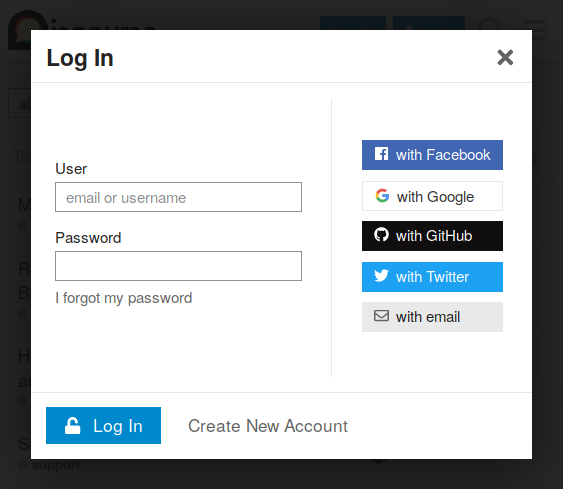
\includegraphics[width=.95\linewidth]{graphics/discourse-sign-in.png}
		\caption{Anmeldung bei Discourse}
		\label{fig:discourse-sign-in}
	\end{subfigure}%
	\begin{subfigure}{.5\textwidth}
		\centering
		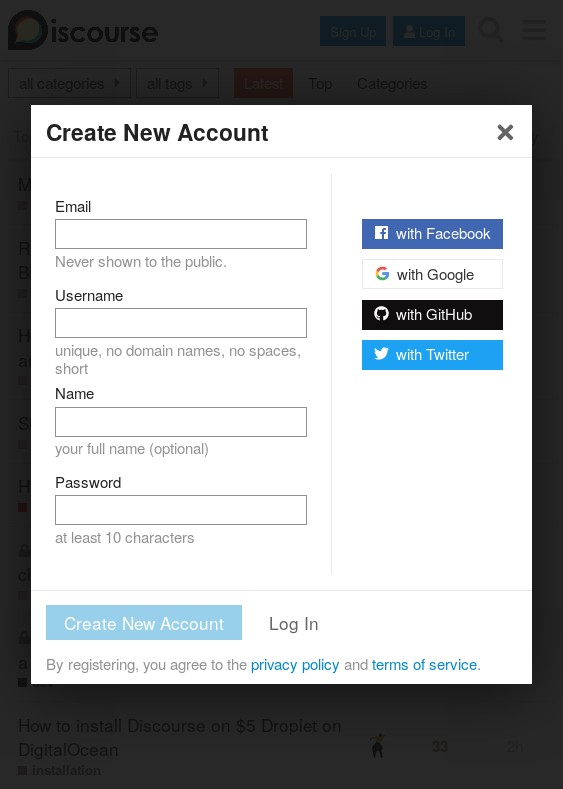
\includegraphics[width=.59\linewidth]{graphics/discourse-sign-up.png}
		\caption{Registrierung bei Discourse}
		\label{fig:discourse-sign-up}
	\end{subfigure}
	\caption{Dialoge zur Anmeldung/Registrierung auf der Webseite Discourse}
	\label{fig:discourse}
\end{figure}

\subsubsection{Dialog Implementierung}
\label{sec:client-dialog-authentication}
Die Anmeldung und Registrierung clientseitig wurden mit einem Dialog-Fenster realisiert. Das Dialog-Fenster\footnote{\url{https://material.angular.io/components/dialog/overview}} wird bereitgestellt von Angular Material. Für die Implementierung eines Dialog-Fensters muss das \enquote{MatDialogModule} eingebunden werden. 

Die von Angular Material bereitgestellten \enquote{tabs}\footnote{\url{https://material.angular.io/components/tabs/overview}} wurden zum dynamischen wechsel der Ansichtsseiten Anmeldung und Registrierung verwendet. Tabs ermöglichen den wechsel zwischen unterschiedlichem Inhalt mit zusätzlicher Animation und gleichbleibender Komponente. Damit \enquote{tabs} verwendet werden können muss das \enquote{MatTabsModule} integriert werden.

Aus diesen beiden Elementen von Angular Material wurde ein Popup-Fenster erstellt, in dem der Wechsel zwischen Anmeldung (Abbildung~\ref{fig:dialog_sign_in}) und Registrierung (Abbildung~\ref{fig:dialog_sign_up}) ermöglicht wird. Bei der Implementierung ist aufgefallen, dass ein Dialog-Fenster im Querformat speziell angepasst werden müsste, da in der hochkant Handyansicht die Darstellung nicht übereinstimmen würde. Ursächlich hierfür ist die im Hochkantformat reduzierte Breite eines Handys.

\begin{figure}[h]
	\centering
	\begin{subfigure}{.5\textwidth}
		\includegraphics[width=.95\linewidth]{graphics/dialog-sign-in.png}
		\caption{Darstellung eines Dialogs zur Anmeldung}
		\label{fig:dialog_sign_in}
	\end{subfigure}%
	\begin{subfigure}{.5\textwidth}
		\includegraphics[width=.95\linewidth]{graphics/dialog-sign-up.png}
		\caption{Darstellung eines Dialogs zur Registrierung}
		\label{fig:dialog_sign_up}
	\end{subfigure}
	\caption{Dialog zur Anmeldung/Registrierung}
	\label{fig:auth-dialog}
\end{figure}

\begin{description}
	\item[Kommunikation mit dem Server]\hfill\\
	Die Kommunikation mit dem Server findet mittels \gls{HTTP}-Anfragen statt. Um eine \gls{HTTP}-Anfrage zu ermöglichen, wird das \gls{HTTP}-Modul von Angular verwendet.

	Während der Arbeit mit Blattwerkzeug, wird ein Entwickler zwangsläufig mit dem Caching-System konfrontiert. Dieses speichert den zuletzt erhaltenen Wert einer \gls{HTTP}-Anfrage. Sollte auf das Observable, welches für die \gls{HTTP}-Anfrage zuständig ist, erneut zugegriffen werden, wird der gespeicherte Wert zurückgegeben. Ein gespeicherter Wert wird erst verändert, sobald explizit eine neue Anfrage an den Server gestellt wird.
	
	Für die Kommunikation mit dem Server wurde mit dem bereitgestellten Caching-System gearbeitet. Damit die zu übermittelnden Daten einer Datenstruktur zugeordnet werden können, wurden Interfaces erstellt. Das Verwenden eines Interfaces als Datenstruktur erleichtert die Identifikation der Zugehörigkeiten der zu übermittelnden Daten. 

	\item[Provider-Buttons]\hfill\\
	Damit zwischen Produktiv-, Entwicklungs-, und Testumgebung unterschieden werden kann, erhalten die Provider Buttons ihre Informationen mittels get Anfragemethode vom Server. Dies bietet den Vorteil, dass serverseitig definiert werden kann, welche Provider dem Benutzer zur Authentifizierung bereit gestellt werden sollen.

	Die Darstellung der Provider-Buttons wird in zwei Komponenten unterteilt. Die provider-button Komponente dient der Darstellung des einzelnen Buttons. Diese enthält jegliche Informationen über den Provider und die Darstellung des Buttons. Die provider-all-buttons Komponente zeigt restlos jeden derzeitig verfügbaren Provider an. Innerhalb der provider-all-buttons Komponente wird auf die provider-button Komponenten zurückgegriffen.
	\item[Validate-Input]\hfill\\
	Der Auth-Dialog beinhaltet verschiedene Input-Felder. Um eine Rückmeldung bei Fehleingabe in einem der Input-Felder zu erhalten, muss ein Input-Feld validiert werden. Hierbei sind verschiedene Möglichkeiten gegeben.

	Die Validierung eines Input-Feldes ist ein fester Bestandteil von \gls{HTML}5. Für eine Validierung mittels \gls{HTML}5 Validator, muss der Validator als Attribut dem Input-Feld hinzugefügt werden. 
	
	Die Angular Validierung bietet bereits vordefinierte Klassenmethoden zur Validierung von Input-Feldern. Die vordefinierten Klassenmethoden gleichen, von der Funktionsweise, den HTML Validatoren. Ein Vorteil den Angular hierbei bietet, ist das Erstellen eigener komplexer Validatoren. Ein weiterer Vorteil, ist das Auslagern der Validatoren aus dem Template. Folglich kann beispielsweise ein Service zur Validierung von Input-Feldern dienen und somit anwendungsübergreifend die Validierung geändert werden.

	Für die Entscheidung zwischen \gls{HTML}5 und Angular Validierung, musste abgewogen werden in welchem Umfang die Validierung benötigt wird. Die zu nutzenden Input-Felder können jeweils mit den vordefinierten Validatoren, beider Validierungs-Möglichkeiten, validiert werden. Aus diesem Grund wurde sich für die \gls{HTML}5 Validierung entschieden, da diese über das Hinzufügen als Attribut eine deutlich komfortablere Lösung bietet.

		Bei der Implementierung der jeweiligen Validatoren innerhalb der Input-Felder wurde erhöhte Code-Redundanz festgestellt. Aus diesem Grund wurde für das Validieren der einzelnen Input-Felder eine validate-input Komponente erstellt. Die validate-input Komponente lädt dynamisch ein Input-Feld mittels ng-content in das Template. Der zu validierende Wert wird mittels input-binding an die validate-input Komponente übermittelt (Listing \ref{lst:validate_input}). Zusätzlich kann mit input-binding das Design des Input-Feldes (Abbildung \ref{fig:validate_input}) erweitert werden. Sollte die Validierung des übermittelten Wertes fehlschlagen, wird undefined an die Eltern-Komponente zurückgeliefert. Dies hat den Vorteil, dass der Client von einem invaliden Wert ausgehen kann und der Server keine invaliden Werte, au{\ss}er undefined, erhält. Allerdings verhindert diese Komponente nur bei falscher Eingabe das Übermitteln von falschen Daten. Aus diesem Grund ist diese Komponente kein Ersatz für die serverseitge Validierung.

	\begin{figure}
		\centering
		\includegraphics[scale=0.7]{graphics/validate-input-example.pdf}
		\caption{Standard und erweiterte Ausführung eines validate-input}
		\label{fig:validate_input}
	\end{figure}

	\begin{minipage}{\linewidth}
			\lstinputlisting[language=JavaScript, style=CodeView, caption=Verwendung einer validate-input Komponente, captionpos=b, label={lst:validate_input}]{snippets/validate_input.ts}
	\end{minipage}
\end{description}

\subsubsection{Speichern eines \gls{JWT}}
Bei dem Erstellen eines \gls{JWT} muss abgewogen werden, wo dieser clientseitig gespeichert werden soll. Hierbei gibt es die Möglichkeit den \gls{JWT} im LocalStorage, sessionStorage oder als Cookie zu speichern.

Der LocalStorage und der sessionStorage sind ähnlich und bieten dieselben Schwachstellen, we{\ss}halb sich im weiteren Verlauf nur auf den LocalStorage bezogen wird. Bei der Speicherung eines \gls{JWT} im LocalStorage wird \gls{XSS} zur Schwachstelle. Bei \gls{XSS} handelt es sich um eine der bekanntesten Angriffsmethoden in der Webentwicklung. Hierbei wird beispielsweise ein Hyperlink manipuliert und mit \JS auf den localStorage zugegriffen. Sobald sich ein Angreifer den \gls{JWT} hat zukommen lassen, ist es für diesen möglich sich mit dem \gls{JWT} zu authentifizieren. Angular schützt seine Applikationen bereits vor \gls{XSS} in dem beispielsweise Eigenschaften und Attribute auf nicht vertrauenswürdige Werte überprüft werden.

Die Speicherung im Cookie bietet die Möglichkeit, mit dem httpOnly-Flag den Zugriff mittels \JS zu verbieten. Zusätzlich kann der secure-Flag gesetzt werden, der die Übertragung des Cookies nur über eine sichere \gls{HTTPS} Verbindung zulässt. Jedoch hat die Speicherung eines Cookies ebenfalls eine gro{\ss}e Schwachstelle. \gls{CSRF} ist ebenso berühmt in der Webentwicklung wie \gls{XSS}. Bei \gls{CSRF} handelt es sich um das Fälschen von Anfragen einer Webseite auf die kein Einfluss genommen werden kann. Dabei wird die Anfrage so gefälscht, dass der Server von einem legitimen eingeloggten Benutzer ausgeht.

Bei der Entscheidung zwischen \gls{XSS} oder \gls{CSRF} muss abgewogen werden, was einem sicherer erscheint. Da sich bei der Verhinderung von \gls{XSS} sehr stark auf Angular verlassen wird, wurde sich für \gls{CSRF} entschieden. Das bedeutet, der \gls{JWT} wird in einem Cookie mit dem httpOnly- und dem secure-Flag versendet.

\subsubsection{Sicherheit und Login}
\label{sec:client-security-login}
Die clientseitige Einstellungsmöglichkeit für Sicherheit und Login kann erst aufgerufen werden, sobald ein Benutzer sich angemeldet hat. Für die Input-Felder wurde die bereits erstellte validate-input Komponente verwendet. Damit zwischen den Einstellungsmöglichkeiten unterschieden werden kann, wurde jeweils eine Komponente erstellt. Da die Einstellungsmöglichkeiten sich auf ein paar wenige einschränken, wurden die erstellten Komponenten in einer Komponente zusammen getragen.

\begin{figure}
	\centering
	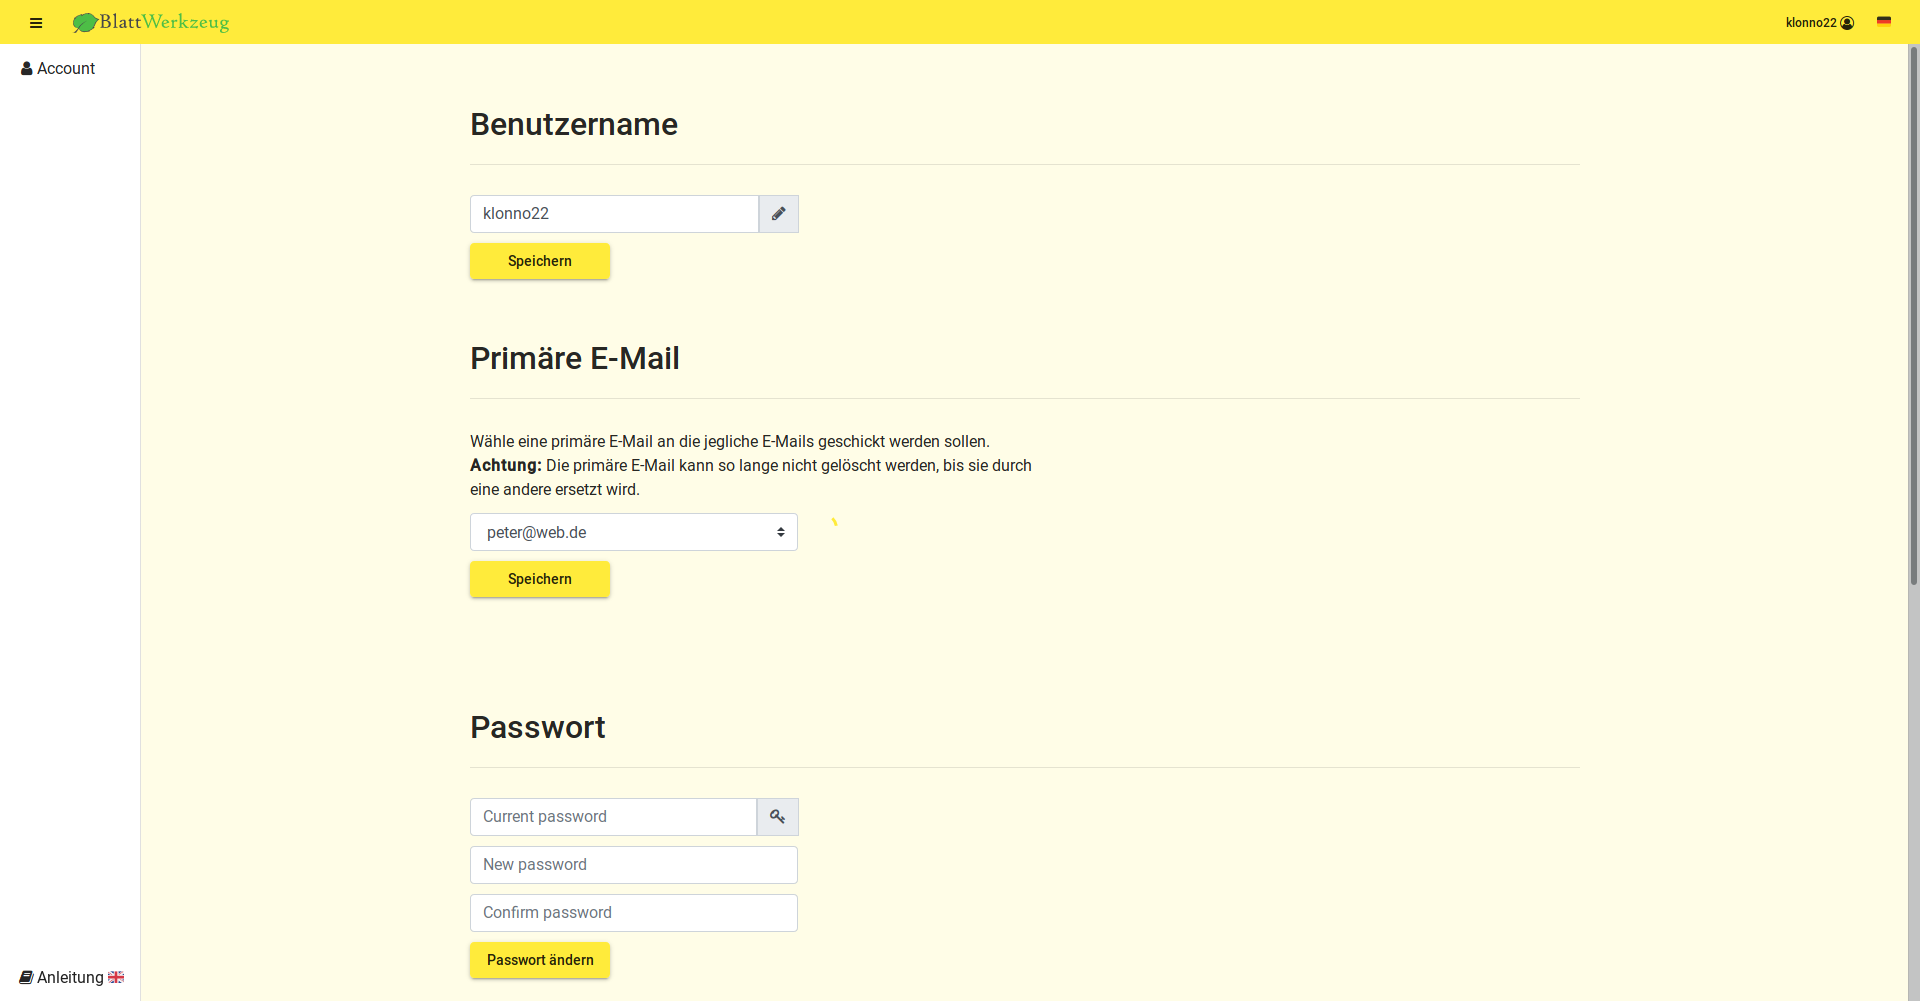
\includegraphics[width=\textwidth]{graphics/account-settings-1.png}
	\caption{Standart und erweiterte Ausführung eines validate-input}
	\label{fig:account_settings_1}
\end{figure}

\begin{figure}
	\centering
	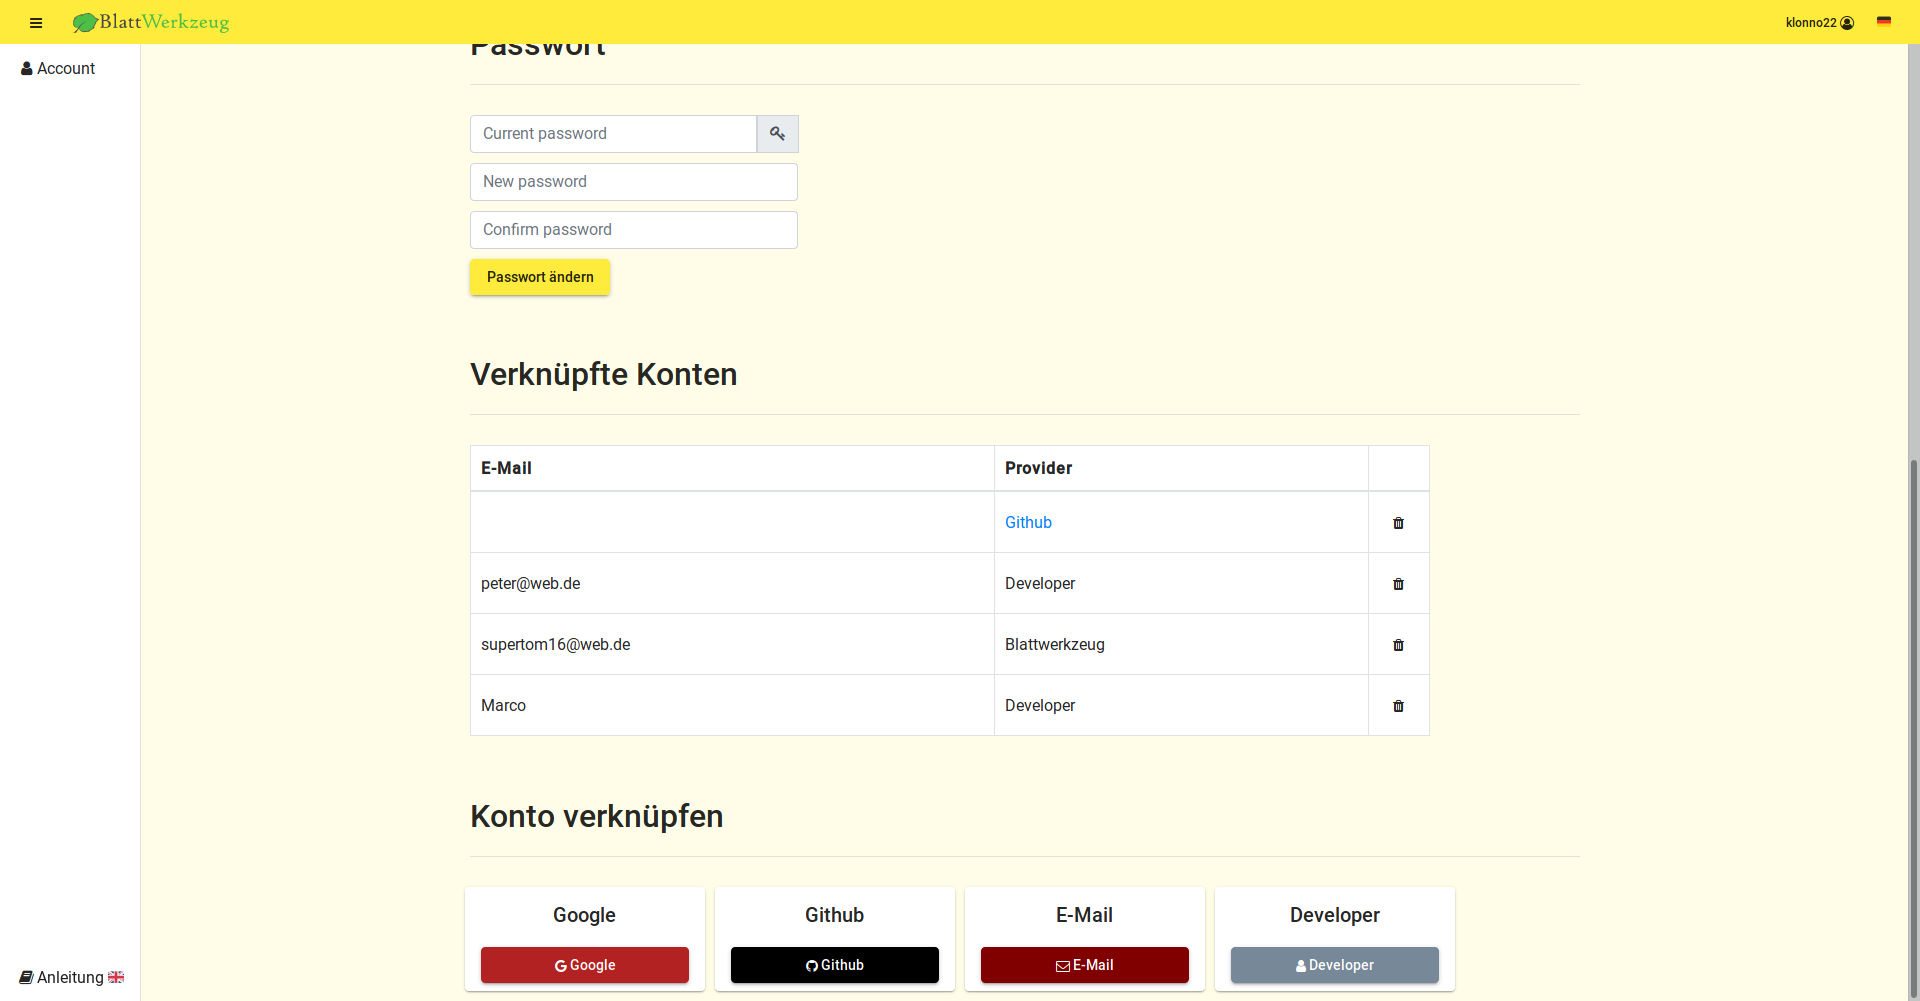
\includegraphics[width=\textwidth]{graphics/account-settings-2.png}
	\caption{Standart und erweiterte Ausführung eines validate-input}
	\label{fig:account_settings_2}
\end{figure}


\begin{description}
	\item[Passwort ändern]\hfill\\
	Sollte ein Benutzer sein Passwort ändern wollen, muss dafür vorerst eine Passwort Identität vorhanden sein. Falls keine Passwort Identität vorhanden ist, wird dem angemeldeten Benutzer keine Passwort Änderung angezeigt. Damit ein Benutzer nicht versehentlich ein falsches Passwort angibt, muss das eingegebene Passwort bestätigt werden.(Abbildung \ref{fig:account_settings_1}) Hierfür muss das neue Passwort erneut eingegeben werden. Damit ein Passwortwechsel erfolgreich durchgeführt werden kann, muss der Server die Eingaben auf ihre Gültigkeit prüfen (Sektion \ref{sec:server-account-settings}).
	\item[Verknüpfte Konten]\hfill\\
	Ein Benutzer soll die Möglichkeit besitzen seine bereits verknüpften Konten zu verwalten. Hierzu wurde eine Übersicht der bereits verknüpften Konten erstellt (Abbildung \ref{fig:account_settings_2}). Diese Übersicht der Konten bietet die Möglichkeit, die bereits verknüpften Konten zu entfernen oder Profilseiten, falls vom Provider ausgeliefert, zu besuchen. Die Entscheidung ob ein verknüpftes Konto entfernt werden darf, obliegt jedoch dem Server (Sektion \ref{sec:server-account-settings}).
	\item[Konto Verknüpfung]\hfill\\
	Damit ein angemeldeter Benutzer sein bereits bestehendes Konto mit weiteren Konto verknüpfen kann, wurden die bereits erstellten provider-button Komponenten zur Darstellung verwendet. Hierbei ist die Funktionsweise in den Einstellungen identisch zu der Funktionsweise des Dialogs (Sektion \ref{sec:client-dialog-authentication}).
\end{description}

\subsubsection{Wrapper-Komponenten}
\label{sec:client-wrapper-components}
Die Darstellung der Blattwerkzeug-Seite muss abhängig von den Rollen eines Benutzers sein. Hierfür ist es möglich, die Unterteilung der einzelnen Codeabschnitte jeweils mit der Angular internen *If Direktive zu lösen. Eine weitere Möglichkeit wäre, die zu den Rollen angepassten Codeabschnitte jeweils in eigene Komponenten auszulagern. Ebenso ist es möglich eine Wrapper-Komponente zu entwickeln, die dynamisch den Inhalt ihres Templates lädt und hierbei bedingt zwischen dem übermittelten Inhalt unterscheiden kann.

Das Nutzen der *If Direktive Angulars für jegliche Codeabschnitte hat den Nachteil, dass erhöhte Coderedundanz ensteht. Jede Komponente die Codeabschnitte abhängig von einer Rolle besitzt, müsste auf die jeweiligen Rollen eines Benuzers Zugriff haben. Dafür müsste in jede Komponente ein Service mit eingebunden werden, der die derzeitigen Rollen eines Benutzers an die Komponente ausliefert.

Die Unterteilung der einzelnen Codeabschnitte in eigene Komponenten hat den Nachteil, dass diese nicht flexibel sind. Eigene Komponenten würden sich stark auf die benötigte Rolle fokussieren. Sollte der Name dieser Rolle geändert werden, müsste nicht nur die Rollen-Abfrage verändert werden, sondern zusätzlich der jeweilige Name der Komponente.

Eine Wrapper-Komponente, die dynamisch ihren Inhalt lädt und gleichzeitig bedingt auf den Inhalt achtet, verhindert erhöhte Coderedundanz und ermöglicht eine einfache Erweiterbarkeit oder Veränderung der Komponente. Aus diesen Gründen wurde sich für diese Methode entschieden.
\begin{description}
	\item[may\_perform]\hfill\\
	Bedienelemente, die von der jeweiligen Benutzerrolle abhängen, wie beispielsweise das Bedienelement zum Speichern eines Projektes, werden mittels der may\_perform Wrapper-Komponente überprüft und dargestellt. Da es sich bei Projekten um Resourcen handelt, die nur bei spezifischer Berechtigung bearbeitet werden dürfen, müssen die Bedienelemente der jeweiligen Resource ausgeblendet werden. Sollten die Bedienelemente weiterhin dargestellt werden, führt dies zu einer schlechten User Experience, da ein Benutzer erst nach der Benutzung des Bedienelementes über eine unzureichende Berechtigung informiert wird. Damit eine Überprüfung serverseitig stattfinden kann, wurde sich vorerst mit den zu übermittelnden Daten beschäftigt. Für die Überprüfung der jeweiligen Funktion eines Bedienelementes, muss der Client die auf dem Server auszuführende Funktion angeben. Hierbei wurde darauf geachtet, dass serverseitig nur Funktionen einer Policy ausgeführt werden können (Sektion \ref{sec:server-authorisation}). Desweiteren benötigt der Server die Informationen auf welcher Ressource diese Funktion ausgeführt werden soll. Sollte es sich bei der Überprüfung um eine spezifische Ressource handeln, muss ebenfalls die ID der Ressource übermittelt werden.
	
	\begin{minipage}{\linewidth}
		\lstinputlisting[language=JavaScript, style=CodeView, caption=Interface der zu übermittelnden Daten, captionpos=b]{snippets/may-perform.ts}
	\end{minipage}
	
	Die may-perform Daten wurden in eine Basisklasse und verschiedene abgeleitete Klassen unterteilt. Dabei beinhaltet die Basisklasse jegliche Daten, die ressourcenübergreifend sind. Die abgeleiteten Klassen beinhalten spezialisierte Daten für eine Resource (Abbildung \ref{fig:client-data-pattern}). Der Service, der zum Aufruf dieser Daten injiziert wird, erstellt beim Aufruf einer Funktion, eine Instanz dieser Klasse. Ein Vorteil dieses Musters ist, dass die Struktur der Daten eindeutig ist, da die abgeleiteten Klassen jeweils einer Ressource entsprechen. Die Funktionen innerhalb des Services werden nach den jeweiligen Resourcen benannt. Daraus resultiert ein eindeutiges Aufruf-Muster, welches den Ressourcen-Namen gefolgt von der Aktion enhält (Listing \ref{lst:client-example_data_pattern}). 
	
	\begin{figure}
		\centering
		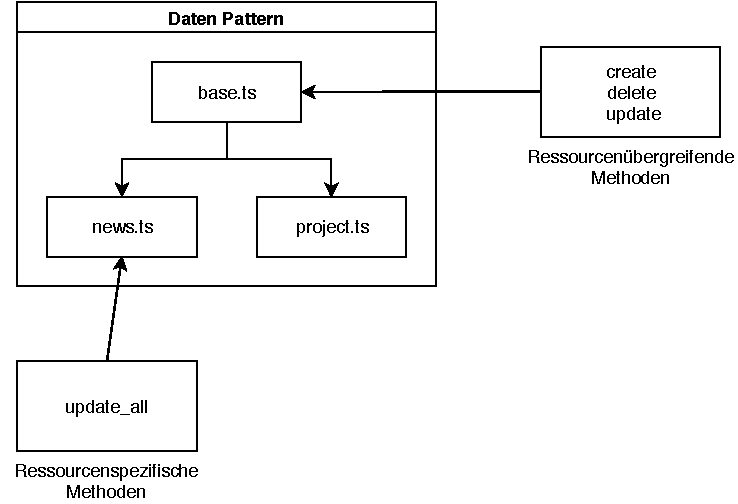
\includegraphics[width=.8\textwidth]{graphics/data-pattern.pdf}
		\caption{Struktur des Daten-Musters}
		\label{fig:client-data-pattern}
	\end{figure}

	\begin{minipage}{\linewidth}
		\lstinputlisting[language=JavaScript, style=CodeView, caption=Beispiel Aufruf zum Erhalten der News-Daten, captionpos=b, label={lst:client-example_data_pattern}]{snippets/example-data-pattern.ts}
	\end{minipage}

	Schlussendlich wird ein Boolscher-Wert an den Client ausgeliefert. Sollte der Boolsche-Wert true zurückliefern, wird das Bedienelement dargestellt.
	
	\item[is-logged-in]\hfill\\
	Ein Besucher erhält  bei einem Aufruf der Blattwerkzeug-Seite Informationen über seinen derzeitigen Benutzer. Die übermittelten Informationen enthalten die Benuzter-Id, die Rollen, die primäre E-Mail und den Benutzernamen. Aus diesem Grund benötigen einige Bedienelemente keine serverseitige Berechtigungs-Abfrage. Das Nutzen  der may-perform Komponente wäre in diesem Fall eine überflüssige Ma{\ss}name, da diese Bedienelemente ausschlie{\ss}lich auf eine globale Rolle geprüft werden.
	
	Die is-logged-in Wrapper-Komponente nutzt die vom Server übermittelten Rollen zur Überprüfung eines angemeldeten Benutzers. Ein angemeldeter Benutzer, wird clientseitig an seiner Rolle identifiziert. Hierfür werden die übermittelten Rollen auf eine guest Rolle geprüft. Das Vorhandensein einer guest Rolle, stellt einen unangemeldeten Benutzer dar. Die Darstellung eines umschlossenen HTML Codeabschnittes mittels is-logged-in hängt von dem derzeitigen Anmeldestatus eines Benutzers ab.  
\end{description}

\subsubsection{Routing-Guards}
\label{sec:routing-guards}
Derzeit ist das Navigieren auf jede Blattwerkzeug-Seite möglich. Routing Guards in Angular bieten die Möglichkeit das Navigieren einzuschränken. Hierfür stellt Angular verschiedene Typen an Routing Guards zur Verfügung. 

\begin{description}
	\item[CanActivate]\hfill\\
	Das CanActivate Interface von Angular wird genutzt um eine bedingte Navigierung zu ermöglichen. Hierbei steht das CanActivate Interface für eine Überprüfung einer aktivierten Route. Eine Route gilt dann als aktiviert, wenn der Routing Guard mit dem CanActivate Interface einen Wahrheitswert zurückliefert. Der Fehlschlag eines CanActivate Routing Guards verhindert jedoch nicht das Laden von Routen gebudenen Modulen.
	\item[CanLoad]\hfill\\
	Das CanLoad Interface von Angular wird für das bedingte Laden von Modulen verwendet. Im Gegensatz zum CanActivate Interface werden Routen gebundene Module beim Fehlschlag eines CanLoad basierenden Routing Guards nicht geladen.
\end{description}

Für die Einschränkung der Navigation auf Blattwerkzeug wurden verschiedene Routing Guards erstellt.

\begin{description}
	\item[AdminGuard]\hfill\\
	Damit Bereiche wie beispielsweise, der Adminbereich, ausschlie{\ss}lich von Administratoren besucht werden können, wurde ein AdminGuard implementiert. Für die Überprüfung des AdminGuards werden die globalen Rollen eines Benutzers auf eine admin Rolle geprüft. Sollte dem derzeitigen Benutzer keine admin Rolle zugewiesen sein, wird dem Benutzer eine Fehlermeldung angezeigt. Die Fehlermeldung wurde mittels Asynchroner-Funktion und einem Dialog-Fenster implementiert. Das Dialog-Fenster bietet die Möglichkeit, mittels afterClosed Funktion, ein Observable als Rückgabewert festzulegen.
	
	Zitat:
	 \begin{quote}
		``Ein Observable ist die Repräsentation einer beliebigen Menge von Werten, die über eine beliebige Zeitdauer verteilt sein könnnen.``\footnote{\url{https://www.buschmais.de/wp-content/uploads/2019/01/01-2019-Java-aktuell_AUTOR_Michael-Ruttka_Einfuehrung-in-RxJS.pdf}}
	\end{quote}

	Das Schlie{\ss}en des Dialog-Fensters löst das zurückgegebene Observable aus. Sobald das Observable ausgelöst wurde, wird auf die Startseite zurück navigiert.
	
	\item[LoggedInGuard]\hfill\\
	Der LoggedInGuard ähnelt in seiner Funktionsweise dem AdminGuard. Allerdings wird dieser Routing Guard zur Überprüfung eines eingeloggten Benutzers verwendet. Die Einstellungen für Sicherheit und Login dürfen beispielsweise ausschlie{\ss}lich als angemeldeter Benutzer eingesehen werden. Sollte ein unangemeldeter Benutzer eine von einem LoggedInGuard geschützte Route besuchen, erhält dieser die Möglichkeit sich vorerst anzumelden. Da der LoggedInGuard sich ausschlie{\ss}lich im Dialog-Fenster und der zu überprüfenden Rolle von dem AdminGuard unterscheidet, wird die Implementierung nicht weiter erläutert.
	
	\item[MasterGuard]\hfill\\
	Bevor der AdminGuard oder der LoggedInGuard fehlschlägt, werden jeweils Dialog-Fenster geöffnet. Sollten mehrere Routing Guards für eine Route festgelegt werden, werden bei dem Fehlschlagen der Routing Guards die Dialog-Fenster übereinander gelegt. Die Ursache dafür ist das von Angular festgelegte, gleichzeitige Ausführen von Routing Guards. Aus diesem Grund muss ein Algorithmus zum Ausführen nacheinander gefolgter Routing Guards implementiert werden. 
	
	er MasterGuard implementiert einen Algorithmus zum Ausführen nacheinander gefolgter Routing Guards. Hierfür werden die auszuführenden Routing Guards im data Objekt des Routes Typen hinterlegt. Sobald der MasterGuard aufgerufen wird, erfolgt über die von Angular übergebene Route ein Zugriff auf das data Objekt. Anschlie{\ss}end wird von jedem, im data Objekt enhaltenen Routing Guard, eine Instanz erstellt und die canActivate Methode aufgerufen. Sollte ein Routing Guard fehlschlagen, schlägt der Master Guard ebenfalls fehl.

\end{description}

%%% Local Variables:
%%% mode: latex
%%% TeX-master: "Tom - Thesis"
%%% End:
